\documentclass[10pt,preprint]{sigplanconf}

\usepackage[utf8]{inputenc}
% the following standard packages may be helpful, but are not required
%\usepackage{longtable}
\usepackage{mathtools}
\usepackage{multicol}
\usepackage{multirow}
\usepackage{booktabs}
\usepackage{courier}
\usepackage[scaled]{helvet}
\usepackage{url}
\usepackage{listings}
\usepackage{enumitem}
\usepackage{mdwlist} % tighter description environment (starred)
\usepackage[colorlinks=true,allcolors=blue,breaklinks,draft=false]{hyperref}
% known bug: http://tex.stackexchange.com/questions/1522/pdfendlink-ended-up-in-different-nesting-level-than-pdfstartlink
\newcommand{\doi}[1]{doi:~\href{http://dx.doi.org/#1}{\Hurl{#1}}}   % print a hyperlinked DOI

\usepackage{graphicx}
\usepackage{softdev}
\usepackage{amsmath}
\usepackage{mdwlist}
\usepackage{pifont}

\lstset{
	basicstyle=\tt\scriptsize,
	xleftmargin=2em,
    framexleftmargin=1.5em,
	numberstyle=\scriptsize\tt\color{gray},
	captionpos=b,
	escapeinside={{<!}{!>}},
}

\begin{document}

\title{An Investigation into the Warmup Behaviour of Various Virtual Machines}
\authorinfo{Edd Barrett}
           {Software Development Team\\ Department of Informatics\\ King's College London}
           {http://eddbarrett.co.uk/}
\authorinfo{Carl Friedrich Bolz}
           {Software Development Team\\ Department of Informatics\\ King's College London}
           {http://cfbolz.de/}
\authorinfo{Laurence Tratt}
           {Software Development Team\\ Department of Informatics\\ King's College London}
           {http://tratt.net/laurie/}

\maketitle


\begin{abstract}
Warmup is magic.
\end{abstract}

\section*{Rough Notes}

XXX what is the hypothesis we are checking? how about "the traditional notion
of warmup is true", which we then reject?


- safety checks
  - are outliers deterministic across different processes? is the behaviour
    generally the same looking?
  - do some checks on other OS, machine architecture, frequency scaling independent

- threats to validity

\section{Introduction}
\label{sec:intro}

Recently there has been a boom in the number of emerging programming language
implementations. Some of the new implementations target already existing
languages (e.g. HHVM~\cite{XXX} and Truffle/JS ~\cite{XXX}), whereas others
target new languages altogether (e.g. Go~\cite{XXX}, Nim~\cite{XXX},
Rust~\cite{XXX} and Dart~\cite{XXX}). Regardless of the design goals of a new
language implementation, there is a shared consensus among language
implementers: that new language implementations must be performant.  This
consensus stems from the fact that the clock speeds of new CPUs have remained
fixed for the last few years. This means that poor program performance can no
longer be overcome by simply using a faster CPU, and thus there is a great deal
of pressure for language implementers to deliver high performance systems.

With this new focus on building fast language implementations, VM and
compiler engineers have started paying close attention to the performance of
their systems. It is now not uncommon for projects to measure performance over
the development life-cycle of their system;  using benchmarking to spot
performance regressions and to take action should they arise. This is a step
in the right direction; commendable perhaps, however benchmarking is not a
trivial subject.

The problem with benchmarking is that there are many different variables that
must be considered. How many iterations should be run? Does running on
different hardware affect the outcome? Does using a different compiler to build
our VM impact performance? Is this benchmark representative of a real program?
The list goes on. Benchmarking is further complicated by \emph{Just In Time}
(JIT) compilation techniques that are often deployed in modern language
implementations. Typically the initial iterations of a benchmark running on a
JIT tend to be much slower than later iterations. This is due to the fact that
the JIT must profile and compile at runtime in order to generate fast code.
The term \emph{peak performance} is often used to describe the point at which
the fast code has been generated, and it is common for experimenters to
disregard data prior to this point when benchmarking.

Although the concept of JIT warmup is widely known, few people have actually
thought in detail about how we should account for these effects when
benchmarking. Commonly, a mean time for a benchmark derived by running a
benchmark a few times (less than 100) in a single process, before ``chopping
JIT warmup''. Although more intricate methodologies have recently
proposed~\cite{XXX}, uptake has been slow, and it is not clear if they
properly account for JIT warmup either.

In this paper we scrutinise benchmarking methodologies and question if we --
as a field -- are correctly measuring the performance of our JIT compilers,
or if we are fooling ourselves by publishing biased results due to a
misunderstanding of warmup behaviours. Our contributions are as follows:

\begin{itemize}
\item We first discuss the traditional notion of warmup behaviours that we have
come to expect from programming language VMs.
\item We describe an experiment designed to measure faithfully the true
warmup behaviours of industry standard VMs.
\item We analyse the results of our experiment in depth, showing a disparity
between the expected and actual warmup behaviours of modern VMs.
\item \edd{We discuss what we need to do about this?}
\end{itemize}


\section{Conceptions of Warmup}
\label{sec:Conceptions of Warmup}

The term ``warmup'' refers to the way in which language runtimes tend to take
time to reach a steady state of peak performance. The term is mostly used when
talking about JIT compilers. A typical VM
with a JIT begins executing a program in a profiling interpreter. Information
gathered through profiling is then used as a heuristic to decide which portions
of the program are good candidates for compilation to fast native code. Once a
candidate has been compiled, the VM uses the fast native code in the future
(instead of the slow interpreter), thus improving performance.  Although
interpretation, profiling and compilation all come with a performance hit,
ideally there should be a point at which the VM has all of the binary code it
needs to execute the whole program natively. At this point, interpretation,
profiling and compilation should no longer occur, and thus peak performance is
met. Between the start of the VM's execution and the point at which peak
performance is met, the JIT is said to be ``warming up''.

\begin{figure}[h!]
\centering
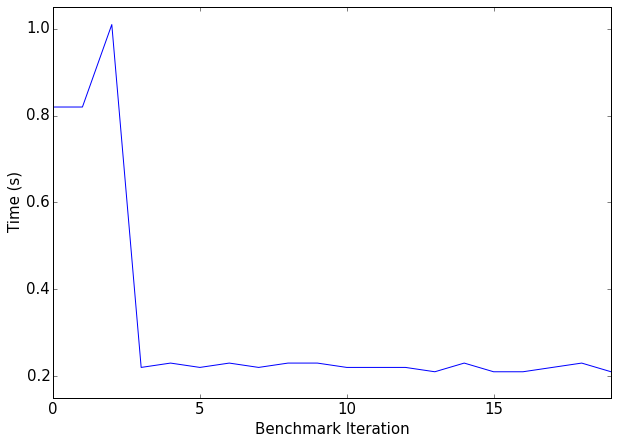
\includegraphics[width=.4\textwidth]{img/trad}
\caption{The traditional notion of JIT warmup impacting a fictional
benchmark running on a fictional VM.}
\label{fig:trad}
\end{figure}

The graph in Figure~\ref{fig:trad} demonstrates the impact that we might
expect JIT warmup to have upon a benchmark running repeatedly within a
single process. In the first iteration (iteration 0), the VM has no compiled
code for the benchmark and therefore it runs slowly in a profiling
interpreter. After two or three iterations the profiler has collected enough
information for the JIT the begin compiling. For this fictional VM,
compilation is more expensive than the profiling interpreter, thus it is
characterised by the spike at iteration 2. \footnote{The cost of
the profiling interpreter relative to that of compilation vary on a per-VM
basis.}At iteration 3, the JIT has compiled all of the code necessary to
efficiently run the benchmark. Subsequent iterations use the compiled code
and therefore run with improved performance. In other words, peak
performance is achieved at iteration 3. Note however that the measured times
for iterations $\geq 3$ are not quite the same. This is because there are many
sources of random variation that impact benchmark measurements. Random
variation can be introduced by the underlying operating system (e.g. by
context switches), or by the VM itself (e.g. garbage collection).  Generally
speaking, we expect peak performance measurements to be fast and ``mostly
constant'', with only small random variations distributed around a constant
mean~\cite{XXX}.  Ideally it would be possible to identify and control the
sources of random variation, allowing us to measure only the performance
characteristics of the VM. In practice however, this is very difficult.


\section{Benchmarking Methodology}
\label{sec:Benchmarking Methodology}

To decide whether expected impact of JIT warmup (as outlined in the previous
section) tallies with reality, we devised an experiment.  The goal of the
experiment is to measure the long-term effects of warmup upon benchmarks,
whilst controlling as many sources of random variation as is practically
possible.

We began with a suite of benchmarks, most of which were collected from Laurence
Tratt's VM experiment~\cite{XXX}. Each benchmark is implemented in multiple
languages allowing us to run them on a range of different VMs. The benchmarks
were modified so as to hook into our benchmark runner, \emph{Krun}. Krun was
originally
developed to run experiments under the Kalibera/Jones
methodology~\cite{XXX}, but since then it has been extended with features to
help measure JIT warmup on Linux. Specifically Krun attempts to address
random variation introduced by:

\begin{description}
\item[Ambient temperature changes] Benchmarks can heat up the system hardware
potentially impacting performance. Krun measures the temperature of the machine
prior to benchmarking, then before starting each benchmark, it waits for the
system temperature to return to within 10$\%$ hotter than the starting
temperature. All temperature zones are checked, and if the system fails to cool
within a resonable time, Krun terminates.\\
\item[Processes sharing the same CPU] Other processes running on the same CPU
as benchmarks can impact performance. Krun therefore insists that benchmarks
are run on an isolated CPU core.~\footnote{We use the \texttt{isolcpus} feature
of the Linux kernel to achieve this. This means that benchmarks share a CPU
only with kernel threads. In theory a core can be fully isolated, however the
Linux tool to enable this is currently broken
(\url{https://bugs.debian.org/cgi-bin/bugreport.cgi?bug=796893})}
\item[The \emph{perf} subsystem] By default, Linux has a kernel profiler,
\emph{perf}, running. This is a significant source of random variation,
especially since it dynamically adjusts (lowers) its sample rate if it is found
to spend too much CPU time. Perf cannot be disabled on X86-64, but Krun insists
that the perf sample rate is set to the lowest possible value of one sample per
second.
\item[CPU governors] Krun attempts to fix the CPU frequency to the highest
possible value (short of overclocking). This is achieved by disabling Intel
p-states support in the kernel and setting CPU governor to \texttt{performance}
mode.~\footnote{This is our best attempt at obtaining a constant CPU clock
speed. The Linux kernel documentation states that ``the idea that frequency can
be set to a single frequency is fiction for Intel Core
processors''~\cite{XXX}.}
\item[Unexpected events] Linux has a tendency to emit important information
relating to system performance to the \texttt{dmesg(1)} buffer. Krun monitors
this buffer, and in the event of a change, mails the experimenter a unified
diff. It is up to the experimenter to decide if the message has impacted
performance.
\item[Heap Usage] The amount of heap memory available to a VM can impact
performance. Krun therefore restricts the amount of heap memory available to
the VM.
\end{description}

We ran the benchmarks on a collection of modern programming language VMs: PyPy
(a meta-tracing VM for Python-2.7); Hotspot (Oracle's Java VM); Graal (Oracle's
next-gen Java VM); LuaJIT (a tracing JIT for Lua); HHVM (Facebook's PHP JIT);
JRuby/Truffle (a Ruby VM usinf Graal/Truffle); V8 (Google's JIT for
Javascript); and CPython (the reference Python implementation). All bar one of
these VMs include a JIT compiler. CPython is a simple interpreter written in C,
that was included as a kind of sanity check (it should not exhibit JIT warmup
characteristics). We ran each benchmark with 2000 in-process iterations,
and repeated this twice for each benchmarking machine involved. We used two
similar X86-64 machines: the first a quad-core i7-4790K running at 4GHz with
an 8MB cache and 24GB of RAM; the second, an Intel i7-4790 running at 3.6GHz
with 8MB of cache and 32GB of RAM. Both machines run Debian 8 and have Intel
Turbo Boost disabled in the BIOS. All VMs were restricted to using at most
2GB of heap. We did \emph{not} force garbage collection after each
in-process iteration of a benchmark.

\section{Results}
\label{sec:Results}

- analysis of the results
  - found regular results
  - anomalies
  - outliers
    - need a definition, n sigma events? outside of the 99\% confidence interval?
  - slowdowns
    - first few iterations are faster than eventual mean
  - cyclic behaviour
    - every n iterations show really regular behaviour
  - late phase changes
    - definition? "I know it when I see it"

\section{Discussion}
\label{sec:Discussion}

  - discussion:
    - need to give up naive definition of warmup
    - unrealistic to get rid of these anomalies
    - some of benchmarking wisdom is wrong in the presence of this stuff


\section{Conclusions}
\label{sec:conclusion}

\bibliographystyle{abbrvnat}
\bibliography{bib}


\end{document}

